\section{AutoEncoders (\textit{AEs})}

\begin{frame}{Постановка задачи}
    Дан неразмеченный датасет $X = \{\boldsymbol{x}_i\}_{i=1}^N$, где $\boldsymbol{x}_i \in \mathbb{R}^D$.

    \textbf{Цель:} Найти сжатое представление $\boldsymbol{z}_i \in \mathbb{R}^M$, $M < D$, такое что восстановленные данные $\tilde{\boldsymbol{x}}_i$ близки к исходным $\boldsymbol{x}_i$.

    \textbf{Подход:} Использование нелинейных преобразований, реализованных нейронной сетью.
\end{frame}

\begin{frame}[allowframebreaks]{Архитектура автоэнкодера}
    \textbf{Encoder:} Нелинейное отображение $f_{\boldsymbol{\theta}}: \mathbb{R}^D \to \mathbb{R}^M$:
    \begin{equation*}
        \boldsymbol{z} = f_{\boldsymbol{\theta}}(\boldsymbol{x}),
    \end{equation*}
    где:
    \begin{equation*}
        f_{\boldsymbol{\theta}} = f_L \circ f_{L-1} \circ \ldots \circ f_1, \quad f_i = \sigma_{\text{E}i}(\mathbf{W}_{\text{E}i}\boldsymbol{z}_{i-1} + \boldsymbol{b}_{\text{E}i}).
    \end{equation*}

    \textbf{Decoder:} Восстановление $g_{\boldsymbol{\phi}}: \mathbb{R}^M \to \mathbb{R}^D$:
    \begin{equation*}
        \tilde{\boldsymbol{x}} = g_{\boldsymbol{\phi}}(\boldsymbol{z}),
    \end{equation*}
    где:
    \begin{equation*}
        g_{\boldsymbol{\phi}} = g_L \circ g_{L-1} \circ \ldots \circ g_1, \quad g_i = \sigma_{\text{D}i}(\mathbf{W}_{\text{D}i}\boldsymbol{z}_{i-1} + \boldsymbol{b}_{\text{D}i}).
    \end{equation*}

    \textbf{Полная архитектура:}
    \begin{align*}
        &\boldsymbol{z} = f_{\boldsymbol{\theta}}(\boldsymbol{x}), \\
        &\tilde{\boldsymbol{x}} = g_{\boldsymbol{\phi}}(\boldsymbol{z}).
    \end{align*}

    \begin{figure}
        \centering
        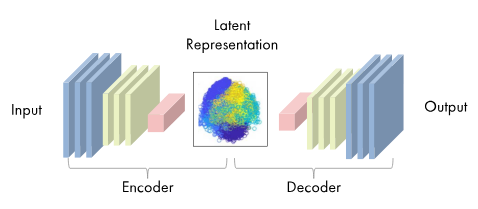
\includegraphics[width=.8\textwidth]{../resources/methods/autoencoder.png}
    \end{figure}
\end{frame}

\begin{frame}{Обучение автоэнкодера}
    \textbf{Функция потерь:} ошибка реконструкции (\textit{reconstruction error}):
    \begin{equation*}
        \mathcal{L}(\boldsymbol{\theta}, \boldsymbol{\phi}) = \frac{1}{N}\sum_{i=1}^N\|\boldsymbol{x}_i - \tilde{\boldsymbol{x}}_i\|^2_2 = \frac{1}{N}\sum_{i=1}^N\|\boldsymbol{x}_i - g_{\boldsymbol{\phi}}(f_{\boldsymbol{\theta}}(\boldsymbol{x}_i))\|^2_2.
    \end{equation*}

    \textbf{Альтернативная функция потерь:} бинарная кросс-энтропия для выхода в $[0, 1]^D$:
    \begin{equation*}
        \mathcal{L}(\boldsymbol{\theta}, \boldsymbol{\phi}) = \frac{1}{N}\sum_{i=1}^N\sum_{j=1}^D\left(x_{ij}\log\tilde{x}_{ij} + (1 - x_{ij})\log(1 - \tilde{x}_{ij})\right).
    \end{equation*}
\end{frame}

\begin{frame}{Аналогия с PCA}
    \textbf{Ошибка реконструкции в PCA:}
    \begin{equation*}
        \mathcal{L}(\boldsymbol{\theta}, \boldsymbol{\phi}) = \frac{1}{N}\sum_{i=1}^N\|\boldsymbol{x}_i - \tilde{\boldsymbol{x}}_i\|^2_2 = \frac{1}{N}\sum_{i=1}^N\|\boldsymbol{x}_i - \mathbf{B}\mathbf{B}^T\boldsymbol{x}_i\|^2_2.
    \end{equation*}

    Если:
    \begin{equation*}
        f_{\boldsymbol{\theta}}(\boldsymbol{x}) = \mathbf{W}_{\text{E}}\boldsymbol{x}, \quad g_{\boldsymbol{\phi}}(\boldsymbol{z}) = \mathbf{W}_{\text{D}}\boldsymbol{z},
    \end{equation*}
    то:
    \begin{equation*}
        \mathbf{W}_{\text{E}} = \mathbf{B}^T, \quad \mathbf{W}_{\text{D}} = \mathbf{B},
    \end{equation*}
    и автоэнкодер эквивалентен PCA.
\end{frame}

\begin{frame}{Практика}
    \begin{figure}
        \centering
        
\includegraphics[width=.3\textwidth]{../resources/overall/Jupyter_logo.png}
    \end{figure}
\end{frame}